\renewcommand{\figurename}{}
\mychapter{R3.05 Chaînes de transmissions numériques (22h30)}{cap:r305} 
\lhead{R3.05 Chaînes de transmissions numériques (22h30)}

\vspace*{0.2cm}%
      \large
      \href{}{\color{black}Enseignant\\M. Angel Abénia}\\%
      \normalsize
\vspace*{0.5cm}%

Le module R3.05 nous a permis de consolider nos notions sur les systèmes de transmissions numériques. Ainsi, nous avons caractérisé la bande passante d'un système inconnu; observé l'effet d'une bande passante réduite sur le débit d'un signal envoyés, et étudié l'effet d'une perturbation sur l'émission d'un signal et comment la mitiger.

\section{Le problème des liaisons synchrones}

Nous avons observé en TP \textit{Travaux Pratiques} que l'immense inconvénient des liaisons à communications synchrones était que le récepteur devaient se synchroniser à la même fréquence d'horloge que l’émetteur afin de se comprendre. Cela en prenant en compte le temps que met le signal à parcourir la distance les séparant (jamais instantané).
\\ \\
Le signal reste compréhensible si l'horloge est très peu désynchronisée, mais le problème reste de pouvoir la synchroniser sur de longues distances car jouant sur l'instant de décision de l'état d'un signal : s'il est décalé, on ne comprendra pas le même message.
\\ \\
Toujours en TP, nous avons observé l'effet du bruit sur la valence \textit{nombre détat significatif que peu prendre un signal}. Au plus le bruit sera blanc élevé, ou la puissance de reception sera faible, au moins nous pourrions comprendre les changements de signaux à fort nombre d'états (nous comprendrons moins les symboles à 16 états plutôt que ceux à 4).
\\ \\
Ainsi, à moins de pouvoir diminuer le rapport signal sur bruit (en augmentant la puissance d'émission ou diminuer l'atténuation du canal), nous pouvons uniquement dégrader notre signal en lui faisant effectuer moins de variations afin qu'elles puissent être mieux interprêtables par le récepteur.
\\ \\
Nous avons étudié tout ceci lors du premier Travail pratique à l'aide d'un message que nous devions décoder.

\begin{figure}[H]
      \centering
      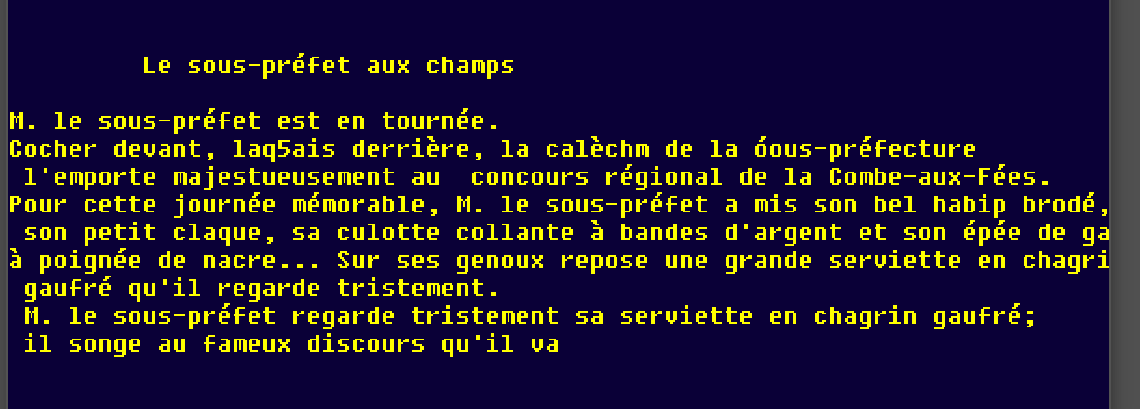
\includegraphics[width=\textwidth - \textwidth / 5]{ressources/r305/00.png}
      \caption{Lecture d'un texte avec une valence de 3 (maximum 3 états significatifs dans notre signal), approuvant nos calculs effectués précedemment comme étant la valence maximale utilisable avec une erreur d'environ 1 bits pour 1000 envoyés.}
      \label{fig:r3051}
  \end{figure}

\begin{figure}[H]
      \centering
      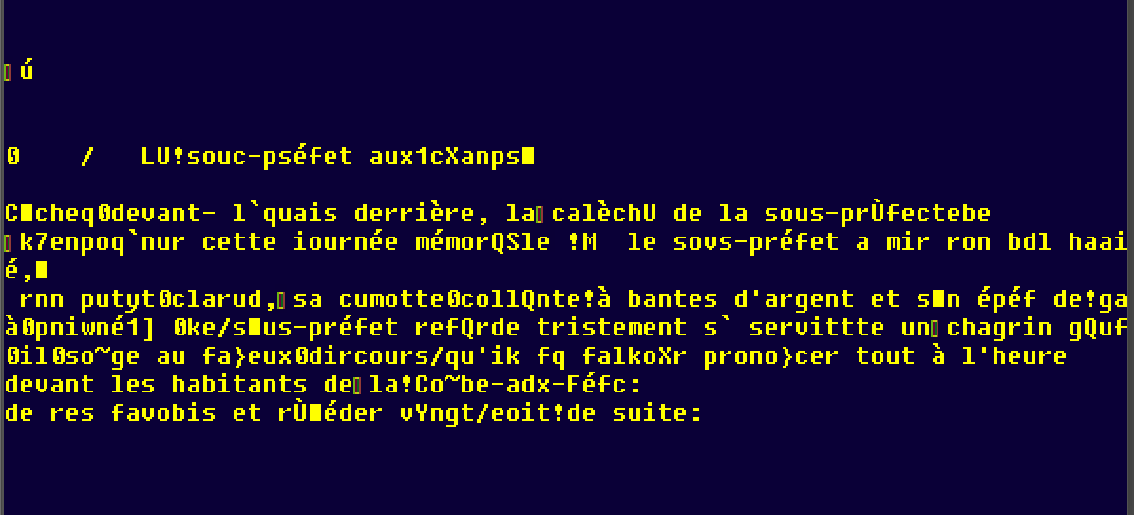
\includegraphics[width=\textwidth - \textwidth / 5]{ressources/r305/01.png}
      \caption{Lecture du même texte avec une valence de 4, le texte est partiellement lisible avec certaines lettres mal interprêtées car les états du signal sont moins reconnaissables, en raison de la valence suppérieure à celle maximale calculée.}
      \label{fig:r3052}
\end{figure}

\section{Étude de l'effet du bruit sur un signal}

Nous avons observé physiquement l'impact du bruit sur un signal. En déhors de décoder un message, nous avons observé que le bruit augmentait le temps que prenait le signal à changer d'états et que ces états étaient moins différenciables plus larges.
\\ \\
L'étude pratique de l'effet du bruit sur un signal peut s'effectuer en observant le diagramme de l'oeil du signal : qui donne les seuils de décision des états du signal et à partir de quand nous pouvons définir qu'un bit est à son état. En voici l'exemple pour un signal à deux états synchronisé parfaitement sur le front montant de l'horloge.

\begin{figure}[H]
      \centering
      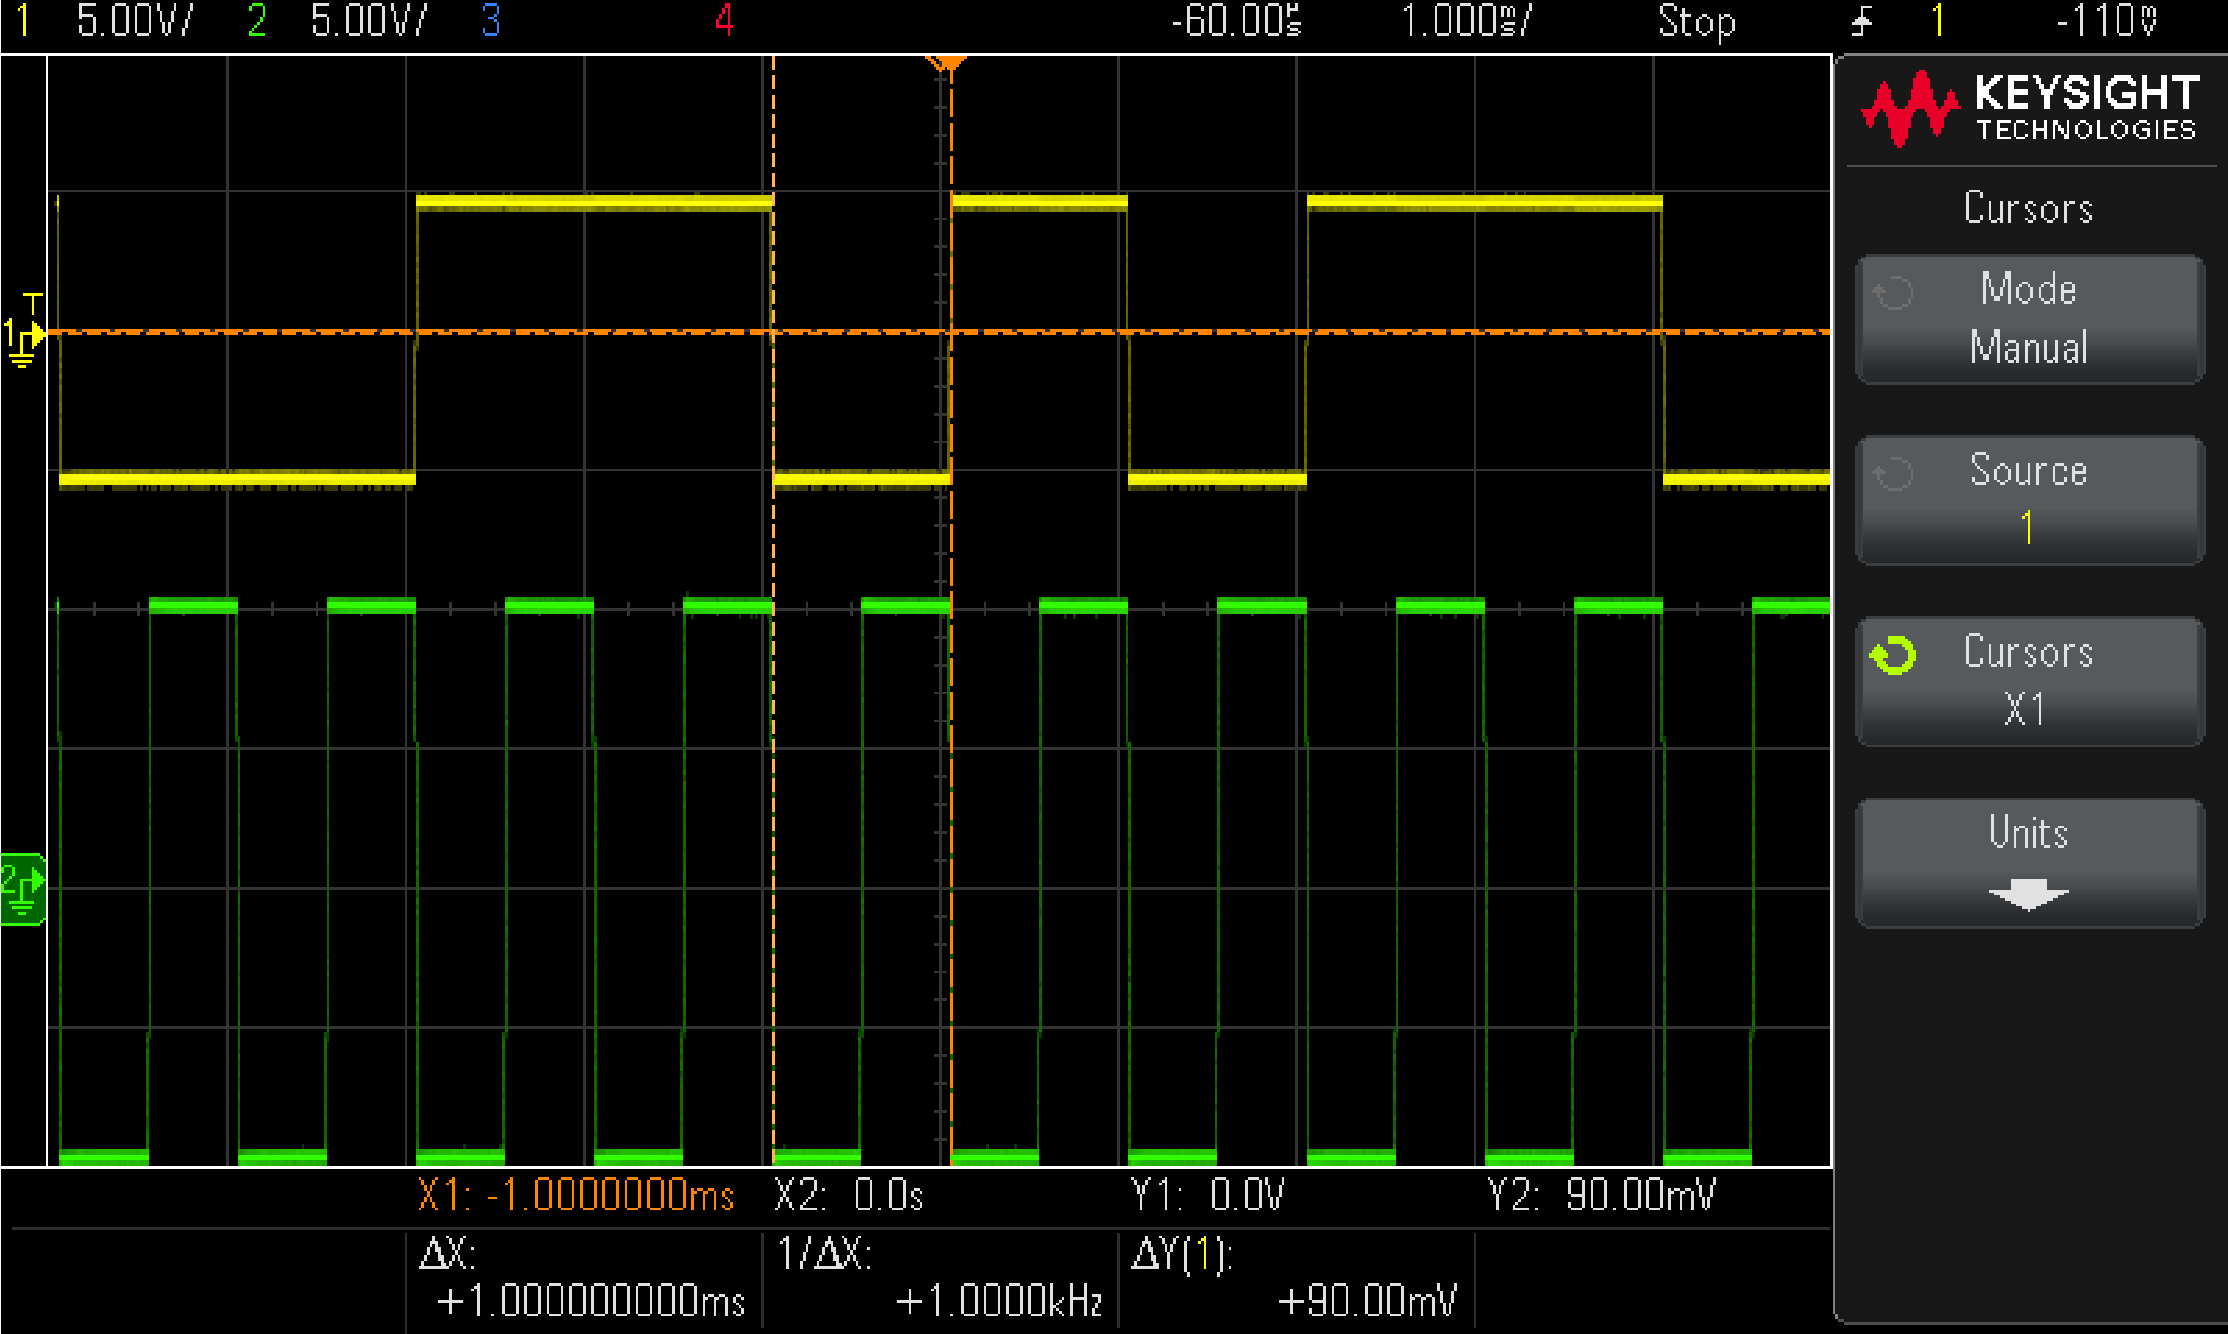
\includegraphics[width=\textwidth - \textwidth / 5]{ressources/r305/02.png}
      \caption{Signal NRZ de 1 ms de temps d'un bit, clocké sur le front montant.}
      \label{fig:r3053}
\end{figure}

\noindent En observant les moments de bascule d'un état 1 à l'état 0, de 0 à 1 et ainsi de suite : nous pouvons voir se former un oeil permettant de définir une plage sur laquelle nous pouvons définir que le signal change d'un symbole pour un autre horizontalement, et à partir de quelle valeur il le fait (verticalement).

\begin{figure}[H]
      \centering
      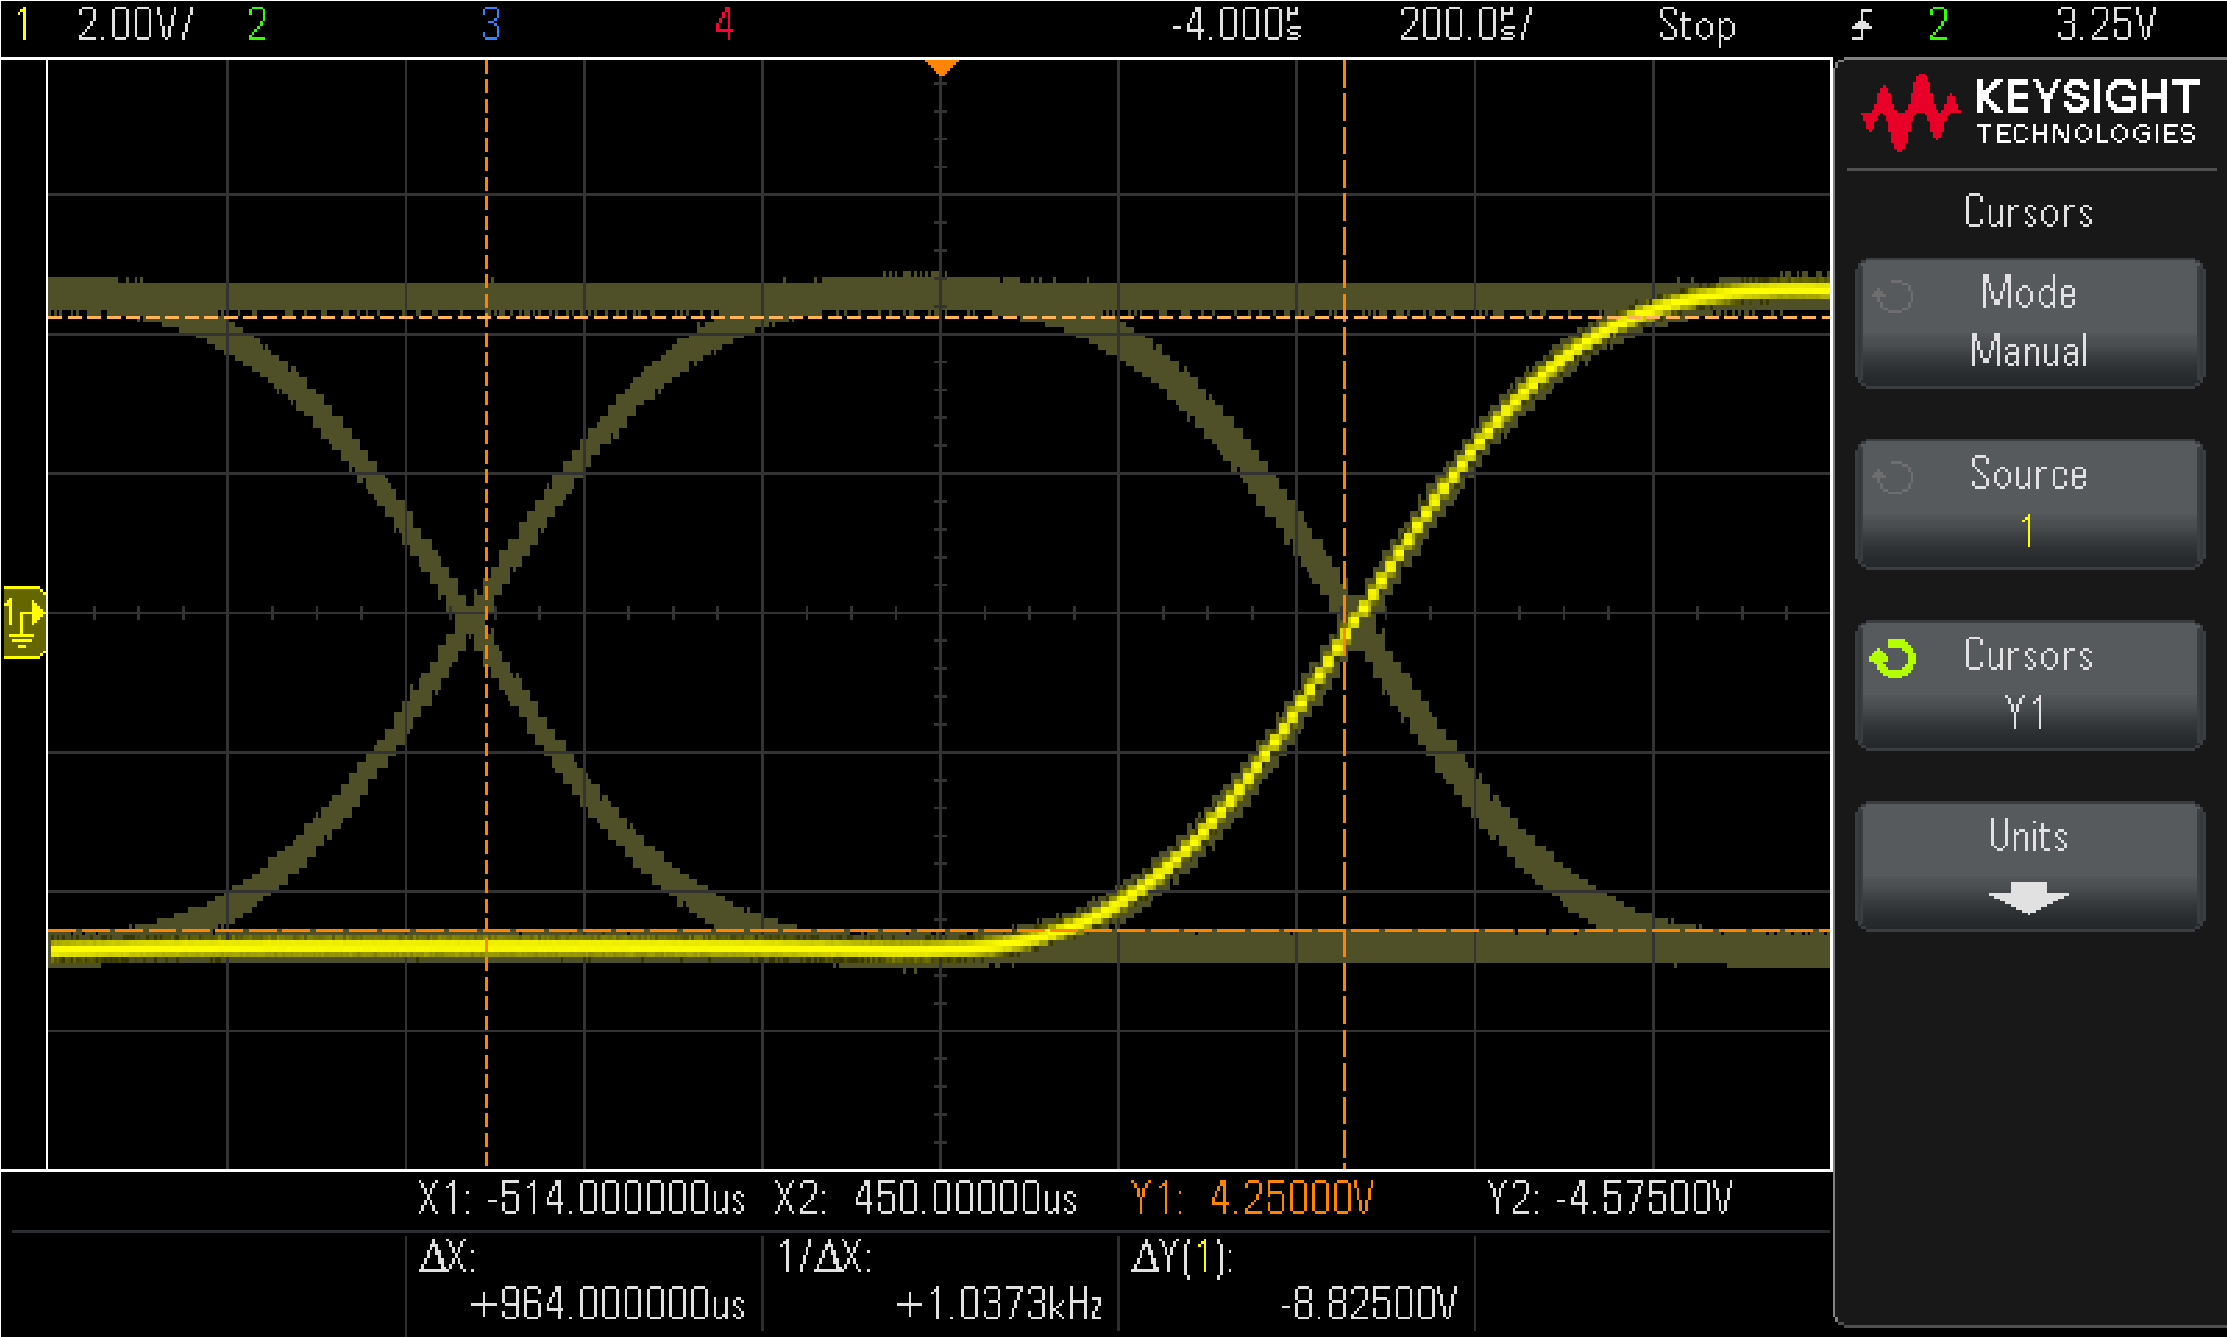
\includegraphics[width=\textwidth - \textwidth / 4]{ressources/r305/03.png}
      \caption{Signal NRZ sur un canal parfait observé avec une plage d'instants de décision de 964 ms (horizontale) et une plage des seuils de décision de 8,825 V centré sur 0 (de 4,25 à -4,5V, vertical) : nous pouvons clairement voir un oeil se dessiner au centre, les valeurs sont extrêmement bien discernables}
      \label{fig:r3053}
\end{figure}

\noindent L'étude était faite à la sortie de l'émetteur, le signal n'était pas rentré dans le support de transmission. Ici le cas pratique de réception de ce signal, avec des états élargis et qui prennent plus de temps à passer d'un état à un autre : le temps où l'ont peut définir quand un bit est à quel état doit changer, aussi l'interval où l'on peut dire qu'il est dans un état ou un autre.

\begin{figure}[H]
      \centering
      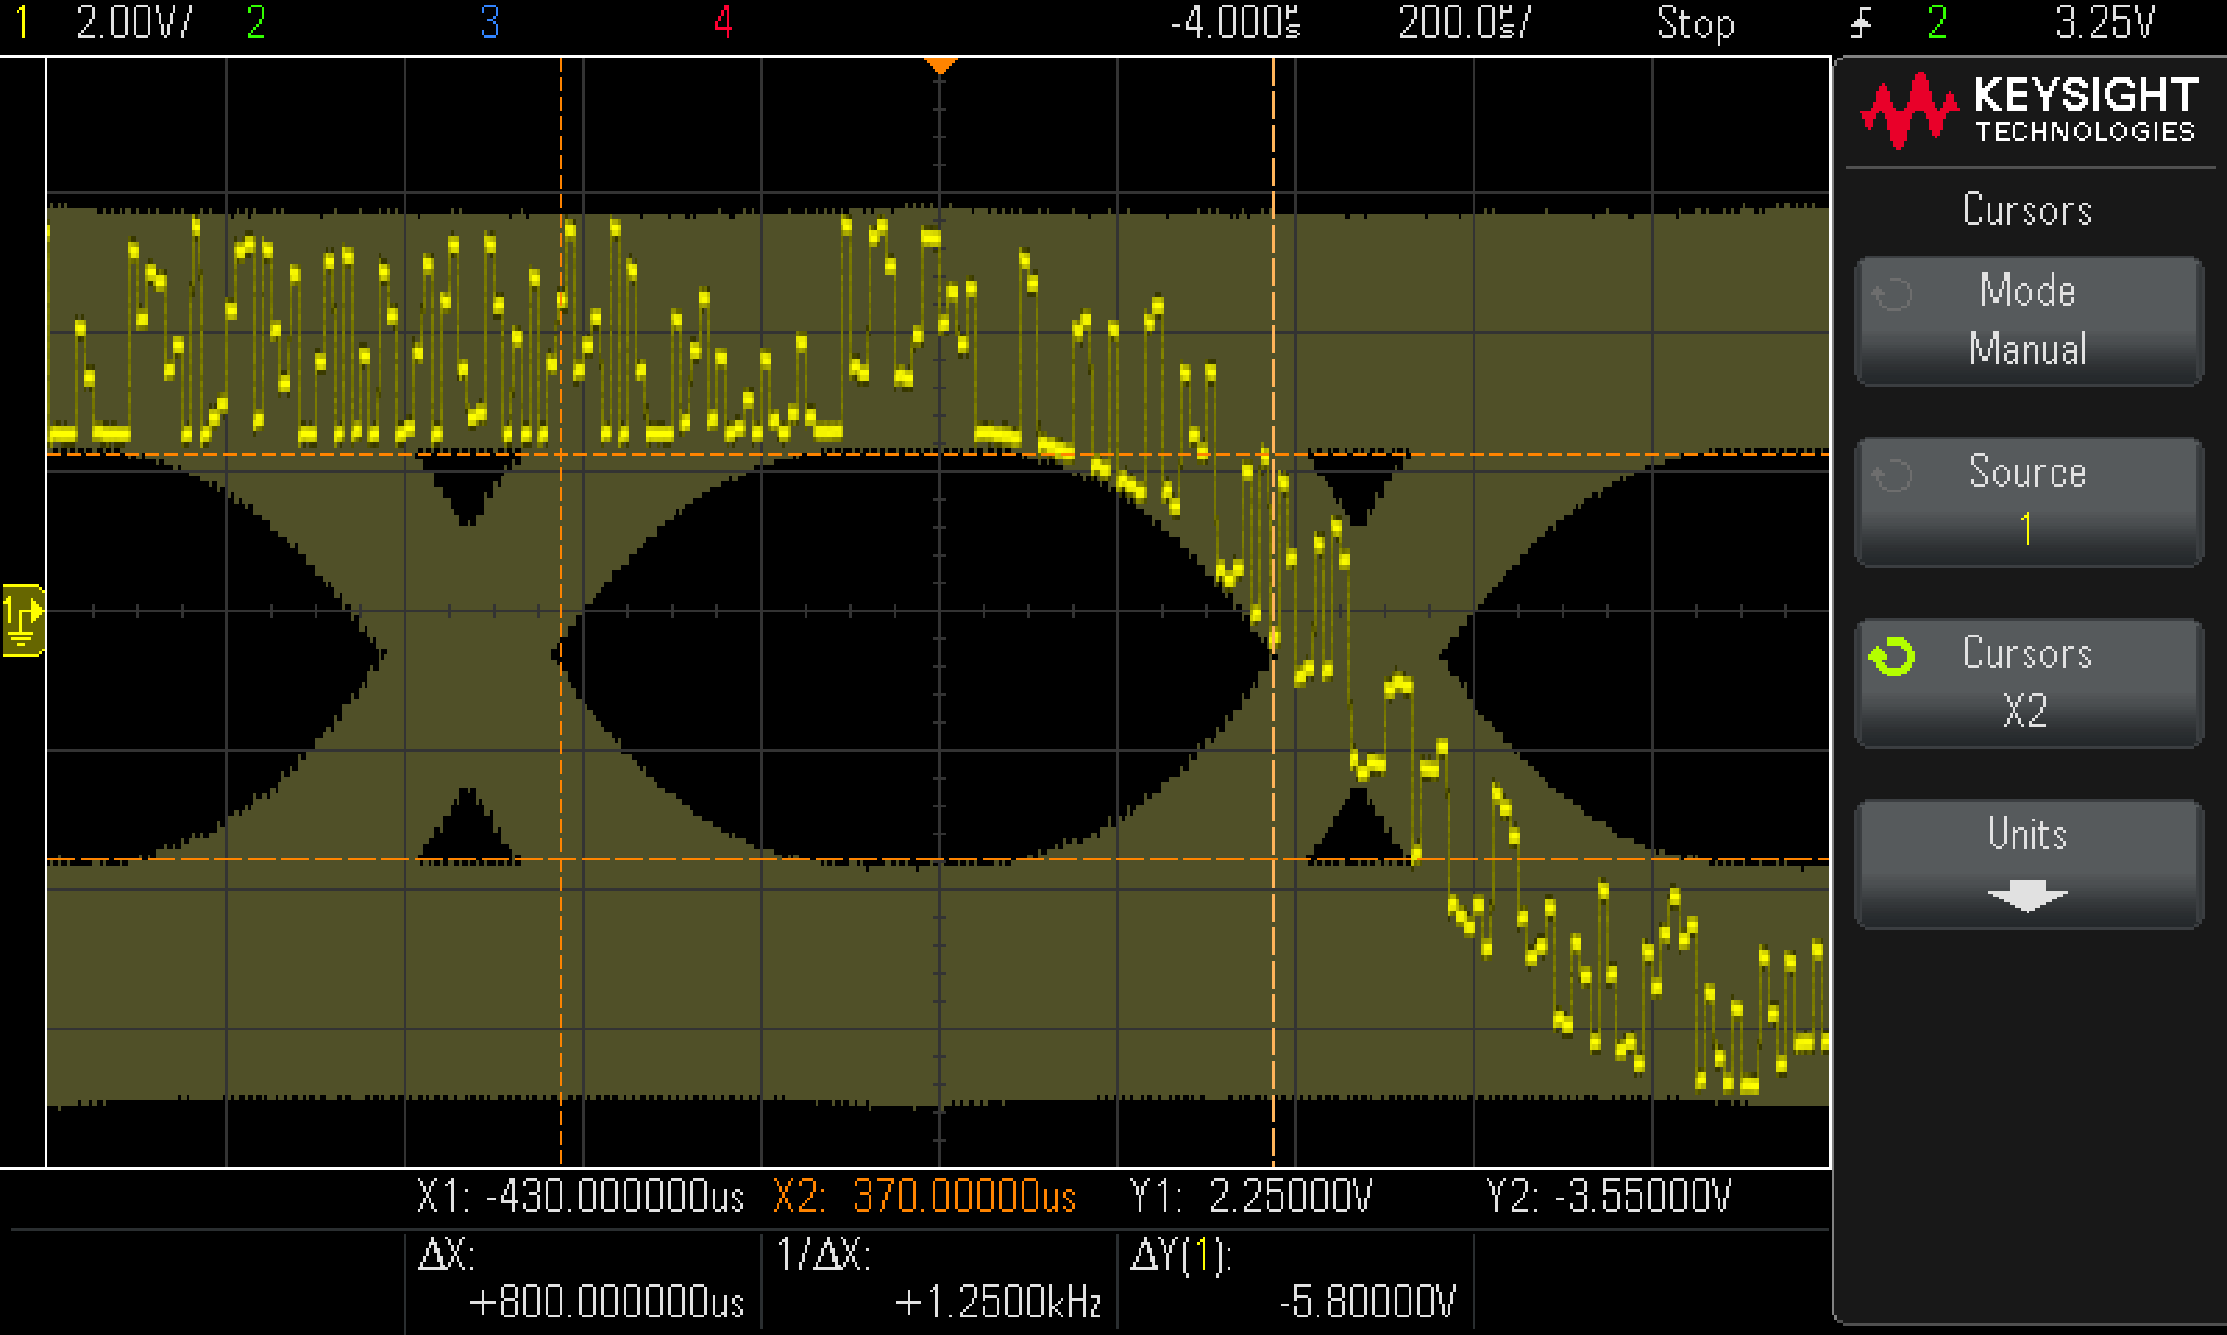
\includegraphics[width=\textwidth - \textwidth / 4]{ressources/r305/04.png}
      \caption{Le signal NRZ est affecté par la bande passante et le bruit du support utilisé, à son extrêmité les états mettent plus de temps à passer d'un état à un autre (plage des instants de décisions réduite à 800 ms entre les deux lignes horizontales) et le bruit fait que les états sont moins discernables (seuils de décisions réduits à 5,8 V entre les deux bandes verticales).}
      \label{fig:r3053}
\end{figure}

\section{Comment minimiser ses problèmes}

Plusieurs solutions ont été inventées pour mitiger ses problèmes au cours du temps. Nous avons étudiés les phénomènes physiques à l'origine de ces solutions afin de comprendre dans quels câdres celles-ci s'inscrivaient et comment elles résolvaient finalement ces problèmes².
\\ \\
Le grand avantage des liaisons à communications synchrones est qu'elles n'ont pas besoin de resynchroniser leur horloge à chaque élément envoyé, ce qui augmente le débit possible de ces mêmes éléments. Leur très grand inconvénient en revanche étant de synchroniser parfaitement les deux horloges si elles sont séparées d'une grande distance.
\\ \\
Ce problème ne se pose pas dans les laisons asynchrones, une synchro-trame \textit{suite de bits que chacun comprend comme le début d'un message} est envoyé avant chaque élément de la conversation. La solution trouvée fut de transmettre l'horloge utilisée dans le message par une fréquence pour se mettre en accord sur la vitesse à laquelle le récepteur devait lire le message. Lui par la suite, en se basant sur les informations envoyées, définit quand est-ce qu'il doit interprêter un état (instants de décisions) pour se placer au milieu d'un état.
\\ \\
Cette solution résout aussi la désynchronisation des horloges : l'électronique n'est pas parfait, les horloges se désynchronisent toujours au bout d'un temps. Le récepteur peut alors regénérer l'horloge de synchronisation car la fréquence y est reçue dans le message. Il peut alors la récupérer, et doit cependant aussi observer les changements d'états du signal pour lui seul se définir les instants de décisions du signal.
\\ \\
Un autre problème de la ligne synchrone est de différencier l'état du signal si celui-ci est inactif pendant un long moment. Avec le codage NRZ par exemple, où les états significatifs du signal sont codés par une valeur électrique : une longue suite de 0 désynchronisera son horloge. Il faut donc en changer le codage utilisé, en choisissant le Manchester par exemple car définit comment est généré son état du signal en se basant sur l'état de celui précédent.